\documentclass[11pt, oneside]{amsart}   	% use "amsart" instead of "article" for AMSLaTeX format
\usepackage{geometry}                		% See geometry.pdf to learn the layout options. There are lots.
\geometry{letterpaper}                   		% ... or a4paper or a5paper or ... 
%\geometry{landscape}                		% Activate for for rotated page geometry
%\usepackage[parfill]{parskip}    		% Activate to begin paragraphs with an empty line rather than an indent
\usepackage{graphicx}				% Use pdf, png, jpg, or epsß with pdflatex; use eps in DVI mode
								% TeX will automatically convert eps --> pdf in pdflatex		
\usepackage{amssymb}
\usepackage{setspace}
\usepackage{enumerate}

\newcommand{\BigO}[1]{\ensuremath{\operatorname{O}\left(#1\right)}}
\newcommand{\BigTheta}[1]{\ensuremath{\operatorname{\Theta}\left(#1\right)}}

\newcommand{\referenceFigure}[1]{Figure [\ref{#1}]}


\title[PCR - Assignment 3 - Moriarty ]{\LARGE{ \bf{ Principles of Cognitive Robotics}} \\ \small{ Homework Assignment 3}}

%\subtitle{this is a sub title}
\author{Alexander Moriarty}
\date{\today}		% Activate to display a given date or no date
\begin{document}
\maketitle
\noindent\textbf{Question 1:}

\noindent\emph{AIMA 3.13 Describe a state space in which iterative deepening search performs much worse than depth-first search (for example, \BigO{n^2} vs. \BigO{n}):}

In a state space where each state has one single successor state, and the goal state is  located at a depth $n$, DFS will arrive at the goal in $n$ steps. Iterative deepening search will however, first need to run through the iterative step until the depth of the search is $n$. In the first iteration it will preform 1 step, in the second it will preform 2, ... until finally the $n^{th}$ iteration where it performs $n$ steps exactly as the DFS. In this case Iterative Deepening Search is performing \BigO{n^2} steps, or \BigTheta{n^2/2}. See \referenceFigure{Figure_1}

\begin{figure}[htbp]
  \centering
  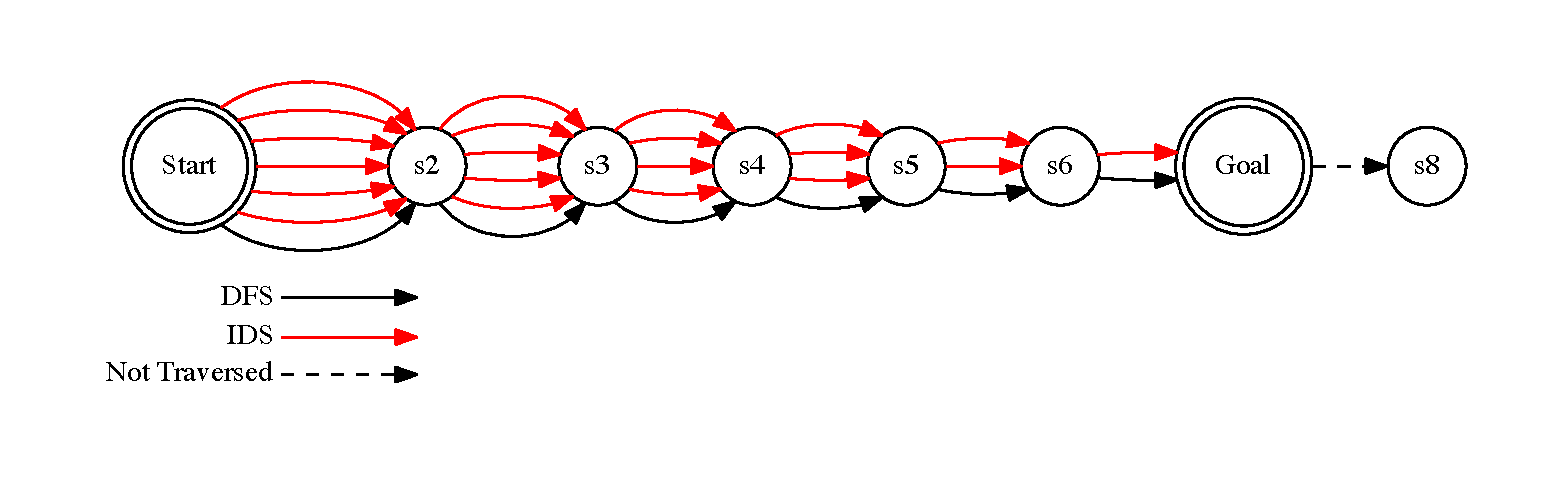
\includegraphics[width=1.0\textwidth]{./media/dfs_vs_ids.pdf}
  \caption{ \label{Figure_1}DFS performs better than IDS in this search space.}
\end{figure}



\noindent\textbf{Question 2:}


\noindent\emph{AIMA 3.15:}
\noindent\begin{enumerate}[a)]


\item If the values of $x$ and $y$ are real, or in $\mathbb{R}$, then they are themselves infinite, even on a finite interval. They are however limited by the  of the computer storing the values $x,y$. Since it clearly states in the problem that this is an `\emph{Idealization}' we shall assume the \emph{ideal} case where we are able to represent all real valued points $(x,y)$ or \emph{states} in this state space. Thus the number of states would be infinite as would the number of paths through the state space from $S$ to $G$.


\item The shortest path from one point, to another point in $n^{th}$ Dimensional space without any obstacles is of course a straight line also in $n^{th}$ Dimensional space... I believe what I am about to say might break down if you can travel from points in $n^{th}$ dimensional space through spaces of higher Dimensions. So it's easy to see that the shortest way from point $A$ to point $B$, or in our case $S$ to $G$ is a straight line. Next we augment this example to have a single line of finite length in the direct path from point $S$ to $G$. A shortest path approach might (ie: bug algorithm) go in a straight line until the obstacle is reached, at which point the agent would be required to turn and follow  the line until one of its end points. But this will create two line segments, basic trigonometry can show that is is faster to travel directly from $S$ to one of the endpoints or \emph{Vertex} of the line obstacle. Now to finally augment this example to the situation of convex polygons is simple. Convex polygon obstacles are nothing more than collections of line segment obstacles which share vertices. 


\item \emph{leaving for later. not allowing external libraries takes the fun out of programming and makes it seem like a tedious waste of time, especially when you know the libraries exist and you would in any real situation use the libraries.} 


\end{enumerate}


\noindent\textbf{Question 3:}


\noindent\emph{AIMA 3.17:}
\noindent\begin{enumerate}[a)]


\item Arbitrarily large negative costs would force any optimal algorithm to exhaustively search the entire state space because with negative costs the exists the possibility of finding an arbitrarily large reward. The Cut Theorem is used in proving most if not all of the optimal search algorithms, it says that if you cut the state space into visited and unvisited states, with the start state being in the visited states and the goal still being unexplored, then the shortest path across the cut will be part of the minimal path. When Negative costs are introduced to the problem, there could exist at the other side of of a non optimal edge a negative cost that will undo taking this non optimal path.


\item In the tree case, it can be shown that a branch will have a maximum reward of the the max negative constant by the remaining depth unexplored $c*depth$. Thus it can be determined if further exploration is required or if a larger reward is not possible and the branch can be pruned from the tree. In the graph case however looping is still possible and the agent can continuously traverse some loop collecting the maximum reward $c$.  


\item If the operators have a negative cost, that is a reward, then it is optimal for the agent to continuously loop collecting the reward. Usually it is desired to prevent this. 


\item Humans generally take continuous numbers of variables into account when making decisions, perhaps there is a nice view but if they have already seen it once or twice already that day, then seeing it again is not as rewarding. Driving the coastal road to the cottage may be beautiful, but it also takes an extra hour. Perhaps the weather that day is not nice and thus the coastal road will be foggy; or the weather is very nice and the reward of getting to the cottage and then to the beach is higher than taking a windy road in a car. It may still be rewarding to take the coastal road every once in a while, especially when there are visitors who haven't seen it also in the car, but otherwise it can seem like a tedious task \emph{(like programming without libraries)}. Artificial agents would need to include memory of having previously visited that state, and receive less of a reward each time it repeatedly revisits a state.


\item There are many reasons to avoid taking an `leap' or a big step. For example, in North America university costs tens of thousands of dollars per year. Going to university will require, entrance into the university plus several part time jobs to pay for the university, and likely a loan from the bank or your parents... and statistically you are still likely to graduate in a debt of tens of thousands of dollars. If you work 3 part time jobs totalling 30 hours per week while attending 15 hours of lecture  and 9 hours of lab plus the ~2 hours of homework per hour of lecture you are left with about 4 hours per day to sleep and do other things. You may be tempted to skip lecture to catch up on sleep. But the costs amount to ~10\$ per lecture hour skipped. You could alternatively not go to university. Instead just directly take a job after high school. The minimum wage (in Canada) varies from ~10 to ~15 \$ per hour. Working full (40hrs/week) time for 49 weeks per year would thus net ~29,000\$ falling into one of the lowest tax brackets. After taxes and living expenses, and then saving (North America is worse at this than Germany) around 20-25 percent of the remaining income, you will be in the black. After 4 years, the minimum time required for a bachelor degree in North America you will have ~11,000 \$. The average student at Dalhousie University graduates with over 35,000 \$ of debt. This cost step has caused a number of my friends from high school to drop out of university, take low paying jobs and thus enter a loop of going to work, getting paid, buying things (big TVs, computers, video games) and going to work.   


\end{enumerate}


\newpage
\textbf{Question 4:}

\emph{The missionaries and cannibals problem is usually stated as follows. Three missionaries and three cannibals are on one side of a river, along with a boat that can hold one or two people. Find a way to get every- one to the other side, without ever leaving a group of missionaries in one place outnumbered by the cannibals in that place.}

\begin{enumerate}[a)]
\item \emph{Formulate the problem precisely, making only those distinctions necessary to ensure a valid solution. Draw a diagram of the complete state space.}

It is necessary to keep for each side of the river the number of monks, cannibals and boats (the boat in this case is a boolean, 0 or 1, but extended versions of this problem exist). Thus six values define a state. There are a number of actions available; however some result in invalid states, where cannibals outnumber monks. The actions can be encompassed in 3 integer values, representing the change in number of monks, cannibals or boats from one site of the river to the other (with the sign indicating direction.)

In the following diagram, the direction of the transition has been ignored for a cleaner graph.

Note: Having error with graphviz, including image and last working version of graph. State spaces accord to those in image
%% 

\item \emph{Implement and solve the problem optimally using an appropriate search algorithm. Is it a good idea to check for repeated states?}

Yes. Without checking for repeated states it is very easy to initially or finally get stuck in loops.

\item \emph{Why do you think people have a hard time solving this puzzle, given that the state space is so simple?}

Because most people take a greedy approach and do not think to bring cannibals or monks back across the river. To many this is a step away from the solution; analogous to being stuck in a local minima while performing a gradient decent to find a global minima.  

\end{enumerate}


\end{document}  